%%%%%%%%%%%%%%%%%%%%%%%%%%%%%%%%%%%%%%%%%
% Journal Article
% LaTeX Template
% Version 1.3 (9/9/13)
%
% This template has been downloaded from:
% http://www.LaTeXTemplates.com
%
% Original author:
% Frits Wenneker (http://www.howtotex.com)
%
% License:
% CC BY-NC-SA 3.0 (http://creativecommons.org/licenses/by-nc-sa/3.0/)
%
%%%%%%%%%%%%%%%%%%%%%%%%%%%%%%%%%%%%%%%%%

%----------------------------------------------------------------------------------------
%	PACKAGES AND OTHER DOCUMENT CONFIGURATIONS
%----------------------------------------------------------------------------------------

\documentclass[twoside]{article}

\usepackage{lipsum} % Package to generate dummy text throughout this template

\usepackage[sc]{mathpazo} % Use the Palatino font
\usepackage[T1]{fontenc} % Use 8-bit encoding that has 256 glyphs
\linespread{1.05} % Line spacing - Palatino needs more space between lines
\usepackage{microtype} % Slightly tweak font spacing for aesthetics

\usepackage[hmarginratio=1:1,top=32mm,columnsep=20pt]{geometry} % Document margins
\usepackage{multicol} % Used for the two-column layout of the document
\usepackage[hang, small,labelfont=bf,up,textfont=it,up]{caption} % Custom captions under/above floats in tables or figures
\usepackage{booktabs} % Horizontal rules in tables
\usepackage{float} % Required for tables and figures in the multi-column environment - they need to be placed in specific locations with the [H] (e.g. \begin{table}[H])
%\usepackage{hyperref} % For hyperlinks in the PDF

\usepackage{lettrine} % The lettrine is the first enlarged letter at the beginning of the text
\usepackage{paralist} % Used for the compactitem environment which makes bullet points with less space between them

\usepackage{abstract} % Allows abstract customization
\renewcommand{\abstractnamefont}{\normalfont\bfseries} % Set the "Abstract" text to bold
\renewcommand{\abstracttextfont}{\normalfont\small\itshape} % Set the abstract itself to small italic text

\usepackage{titlesec} % Allows customization of titles
%\renewcommand\thesection{\Roman{section}} % Roman numerals for the sections
%\renewcommand\thesubsection{\Roman{subsection}} % Roman numerals for subsections
\titleformat{\section}[block]{\large\scshape\centering}{\thesection.}{1em}{} % Change the look of the section titles
\titleformat{\subsection}[block]{\large}{\thesubsection.}{1em}{} % Change the look of the section titles

\usepackage{fancyhdr} % Headers and footers
\pagestyle{fancy} % All pages have headers and footers
\fancyhead{} % Blank out the default header
\fancyfoot{} % Blank out the default footer
\fancyhead[C]{Autonomous Systems Engineering} % Custom header text
\fancyfoot[RO,LE]{\thepage} % Custom footer text

\usepackage{graphicx}
\usepackage{multicol}
\usepackage{tikz}
\usepackage{textcomp}
\usepackage{wrapfig}
\usepackage{floatflt}
\usetikzlibrary{shapes}
% Quellcode
\usepackage{listings}
\lstloadlanguages{C++,Python}
\definecolor{mygreen}{rgb}{0,0.6,0}
\definecolor{myblue}{rgb}{0,0,0.8}
\lstset{ %
	breaklines=true,
	basicstyle=\fontsize{10pt}{12pt}\ttfamily,
	commentstyle=\color{mygreen},
	keywordstyle=\color{myblue},
	rulecolor=\color{black},
	captionpos=b,
	language=Python,
	numbers=left,
	xleftmargin=2em,
	numberstyle=\tiny,
	framexleftmargin=1.8em,
	%numbersep=10pt,
	frame=L}
%----------------------------------------------------------------------------------------
%	TITLE SECTION
%----------------------------------------------------------------------------------------

\title{\vspace{-15mm}\fontsize{24pt}{10pt}\selectfont\textbf{Scenario and Evaluation Algorithms}} % Article title

\author{
\large
\textsc{Hendrik Oestreich, Andreas Gatting, Timo Michalski, Julian Daberkow}\\
\textsc{Julian Exner, <further Authors>}\\%\thanks{A thank you or further information}\\[2mm] % Your name
\normalsize University of Bielefeld \\ % Your institution
%\normalsize hoestreich@techfak.uni-bielefeld.com%\href{mailto:hoestreich@techfak.uni-bielefeld.com}{hoestreich@techfak.uni-bielefeld.com} % Your email address
%\vspace{-5mm}
}
\date{July 2015}

%----------------------------------------------------------------------------------------

\begin{document}

\maketitle % Insert title

\thispagestyle{fancy} % All pages have headers and footers


%----------------------------------------------------------------------------------------
%	ARTICLE CONTENTS
%----------------------------------------------------------------------------------------

%\begin{multicols}{2} % Two-column layout throughout the main article text

\section{Scenario}
\subsection{Teleworkbench}
The teleworkbench (TWB) is a laboratory for evaluation and tracking purposes of mutli-robot scenarios in the CITEC of the University of Bielefeld. An area of 6x6m is tracked by a camera array of 4 cameras mounted at the ceiling. The rest of the room is workspace and used for controlling the experiments in the testing area. 

\subsection{Setup} % TODO Hendrik
Our first task was to build up a setup, to transform the testing area in some kind of an artificial living room. We designed the setup in one of the courses all together. Another week when a few vacuum cleaning robots had arrived, we started to transform our design sketch into reality in the teleworkbench.
For the implementation it was important to avoid covering of areas, because the tracking from the ceiling would fail, if it is not able to see the robot when it is driving under a table.
For this reason the chair legs were only cardbord rolls and we used only the table frame. In Fig. \ref{fig:panorama} you see a panorama photo showing most of the challenges we included in our scenario. 
\begin{figure}[H]
	\centering
	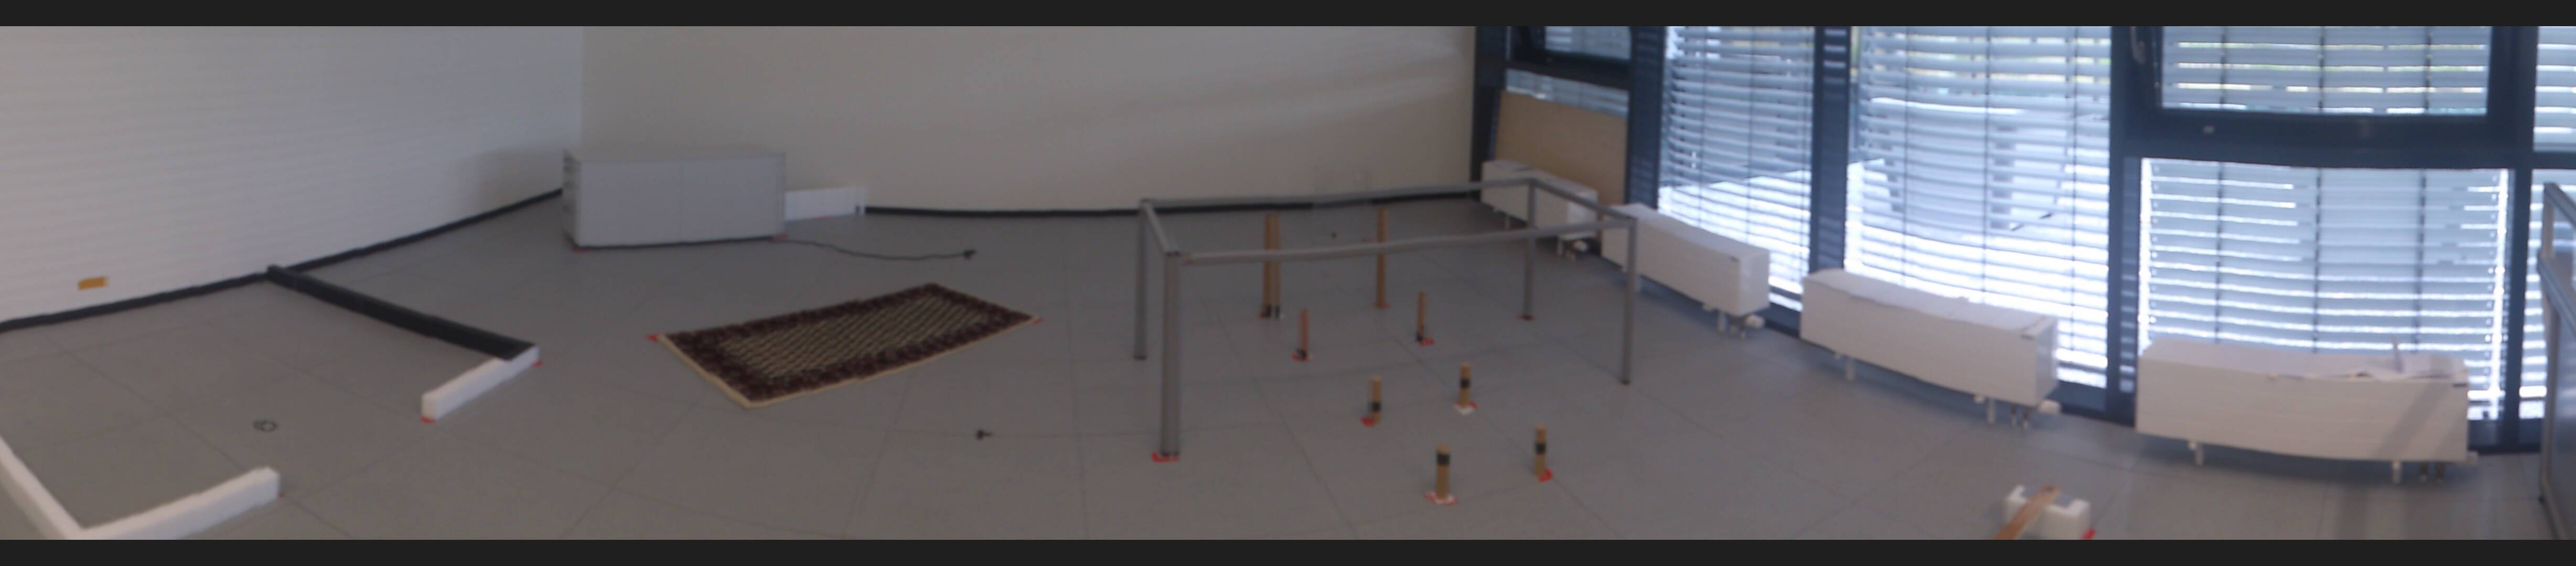
\includegraphics[scale=0.09]{pictures/Setup_panorama.JPG}
	\caption{180$^\circ$ panorama picture of the setup}
	\label{fig:panorama}
\end{figure}
\noindent
In Fig. \ref{fig:scenario} you can see the setup stitched from the cameras at the ceiling and an overlay with the digitized scenario. The following enumaration provides detailed information about the marked positions:
\begin{enumerate}
\item Starting position: The starting position should be equal for all robots. Therefore the charging station was always placed at the position in the middle-bottom of the picture. This guarantees that the robots should all have the possibility to drive straight through the room after leaving the charging station at the beginning of the experiment. Left and right to the starting position the other robots wait in their charging station.
\item Small room: The small room offers at least three challenges. One challenge is the finding of the entrance of the room to simply test if the room is not left out while cleaning the rest of the area. Another challenge was the fact that the room might not allow to see the charging station from the inside what might perhaps produce unpredictable behavior in that case. The last challenge of the rooms was that some walls were white and some were black which could also lead to different treatments depending on the sensors which the robots use. 
\item Clearance height test: This obstacle should be a test if the robots recognize obstacle which they might not fit under. In fact in our case the obstacle was high enough that all robots were able to drive underneath without touching the obstacle. It would have been better if the obstacle would haven been adjusted individually to each robots height.
\item Small chair: We placed to chairs underneath our table to test the navigation in areas were the robots have lots of obstacles around them, which they should not touch or move around. The distances between the front and the back chair legs of the small chair do not allow any of the robots to get between them. They can only reach the area between from one of the sides (left/right).
\item Big chair: The big chair should test the same reactions as the small chair. The only difference is, that the distance between the individual legs allows the robots to get between them from all sides and also clean that area. 
\item Table: The table completes a stereotypical situation which will be part of most living rooms in the real world.
\item Carpet: The carpet is a real challenge for all of the robots. On the one side the robots have to overcome a height difference and on the other hand the material of the ground changes which may result in different driving characteristics. 
\item Loose cable (with fixated ends): Although in most of the manuals the user is advised to make sure that no loose cables may harm the robot in its cleaning area, we decided to include this in our scenario because it will often be the case in the real world and we wanted to investigate the behavior with this kind of obstacles.
\item Trap: The trap only offers a small entrance and may be a problem for robots which only use bump-sensors for navigation because it may take a while for them to get out of this area again. Therefore we also wanted to measure the time which the robot spends inside the trap.
\item Glass cylinder: The material of this obstacle may be challenge for some kind of sensors which the robots use. We wanted to examine whether some robots bump against the cylinder or perhaps even move it around.
\item Heaters: The heaters were given obstacles in the room but they also provided some clearance height test and especially the heating controls turned out to be a problem for some of the robots.
\end{enumerate}
\begin{figure}[H]
	\centering
	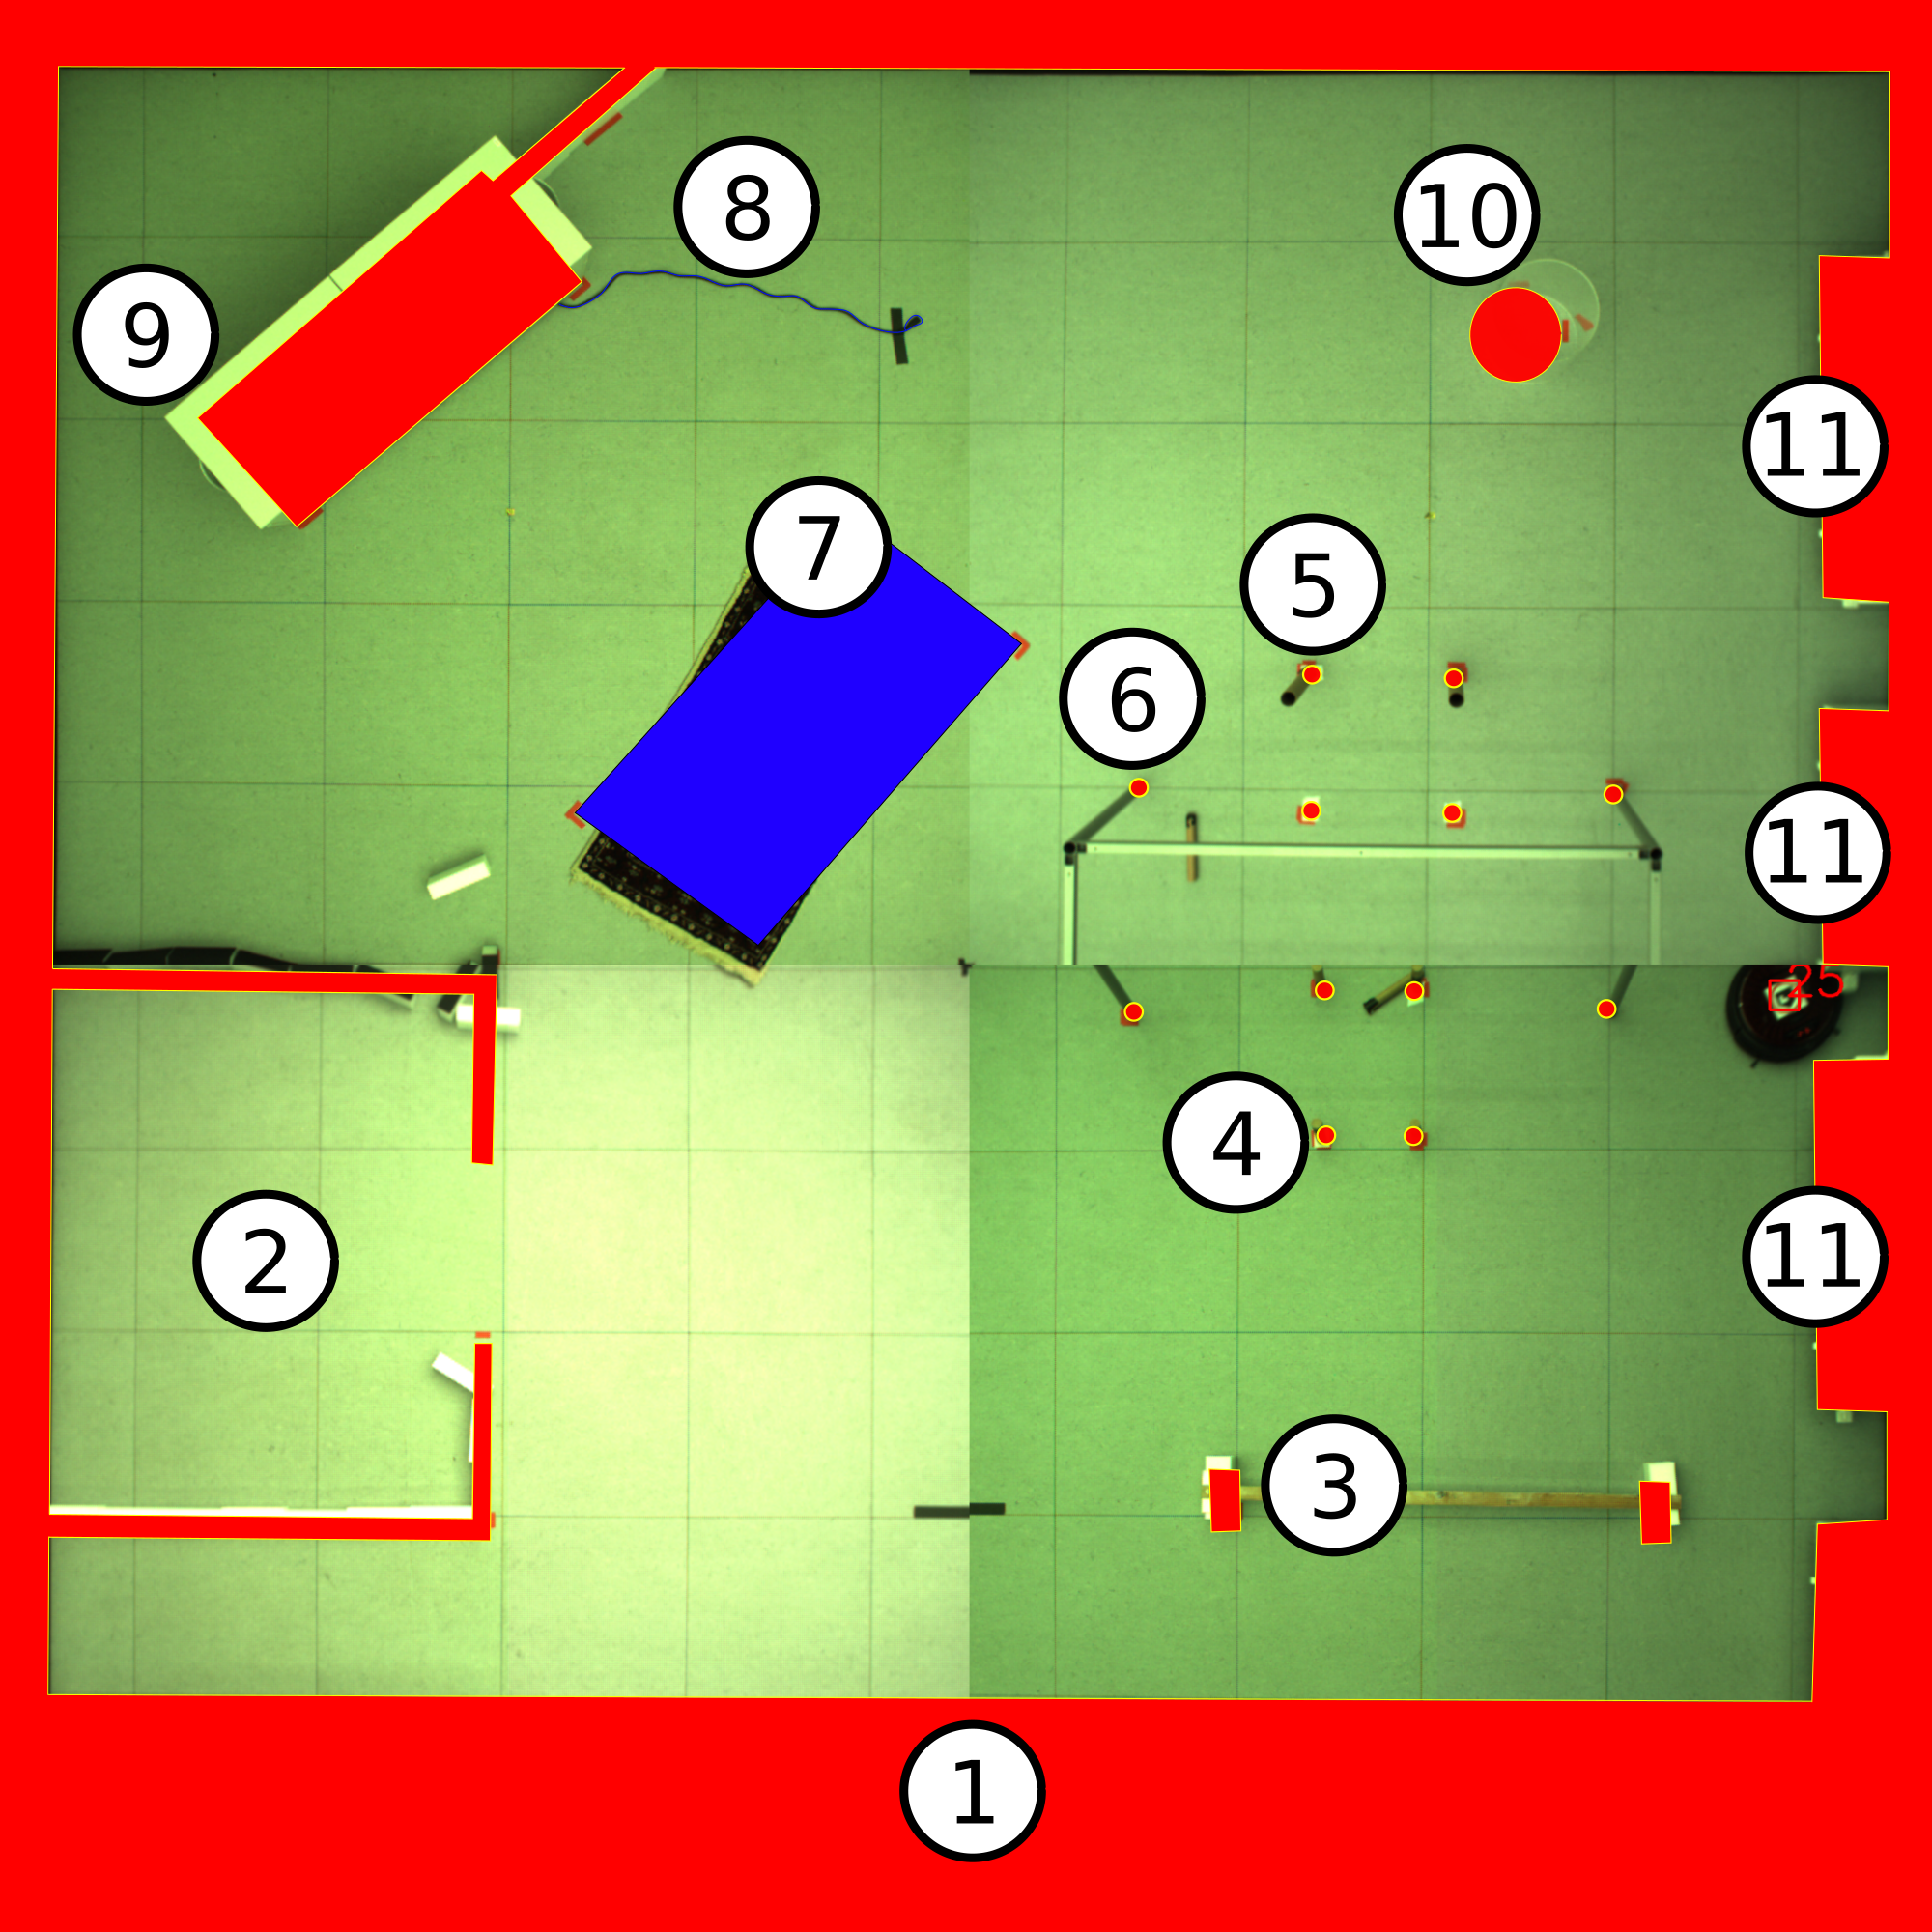
\includegraphics[scale=0.15]{pictures/senario_with_walls_picBack_labels.png}
	\caption{Sketch-overlay of the setup}
	\label{fig:scenario}
\end{figure}
\subsection{Tracking Tool} % Someone else
\subsection{Execution} % TODO Andi

\section{Evalution Algorithms}
\subsection{Group 1}
\subsubsection{Preprocessing of tracking data} % TODO Hendrik
The tracking data came from an external application and consisted of four simple textfiles with the following format for each line:
\[(Time:HHMMSS.MS) (\#Tracked markers) [(Tracker ID) (Angle) (X-Position) (Y-Position)] \]
Which looks like this for a concrete case:
\begin{center}
\texttt{222202.405827\ 1\ 32\ 270\ 87\ 897}
\end{center}
Our first task though was to combine the data from all four text files and create one representation which contains the tracking data relative to the complete area. 
We decided to use a \texttt{QMap} for that because it is an ordered combination of a key and a value. In our case the key is the complete timestamp and the values are vectors which contain the angle and the x and y position. This way it was easy to combine the tracking data in one representation because we could assume that nearly no timestamps are equal and if they are, their tracking data should be very similar so that storing only one of them should be sufficient.
Our approach was to successively iterate over all lines of the four files and then check whether the line holds meaningful data. If it does the values from the line are extracted with simple string operations and depending on the file where they were coming from, an offset is added to the x or y position or to both. At the end of the extraction we had all we need: A timestamp for the key and the relative position and orientation (not needed any further) for our vector.
Later we added a scaling factor to the x and y position because the tracking data does not provide values between the full range from 0-1000. This results from the fact that the pictures for the tracking data are stitched together and because the overlap the tracking data can not reach its maximum values. The scaling factor is multiplied to the x and y positions before adding the offset.
All this is done in the method \texttt{extractData(QMap<qulonglong, QVector<int> > *trackingData, QString filename, int xOffset, int yOffset)}. It is called four times (for the four files) from the method \texttt{preprocessTrackingData()} inside the \texttt{VacCleanAnalyzer} class.
\subsubsection{Distance} % TODO Andi
\subsubsection{Duration} % TODO Timo
\subsubsection{Coverage} % TODO Julian D.
\subsubsection{Heatmap} % TODO Leroy

\subsection{Group 2} % TODO Julian E. & Martin
\subsubsection{Preprocessing of tracking data}
\subsubsection{Heatmap}
\subsubsection{Histogram}

%\end{multicols}

\end{document}
